\documentclass{article}

% set font encoding for PDFLaTeX or XeLaTeX
\usepackage{ifxetex}
\ifxetex
  \usepackage{fontspec}
\else
  \usepackage[T1]{fontenc}
  \usepackage[utf8]{inputenc}
  \usepackage{lmodern}
  \usepackage{graphicx}
  \usepackage{float}
\fi

% used in maketitle
\title{Atmósfera Terrestre}
\author{Eduardo Hernández Sánchez}
\date{25 Enero 2018}
% Enable SageTeX to run SageMath code right inside this LaTeX file.
% documentation: http://mirrors.ctan.org/macros/latex/contrib/sagetex/sagetexpackage.pdf
% \usepackage{sagetex}

\begin{document}
\maketitle
\section{Atmósfera Terrestre}
\begin{figure}[h!]
\centering
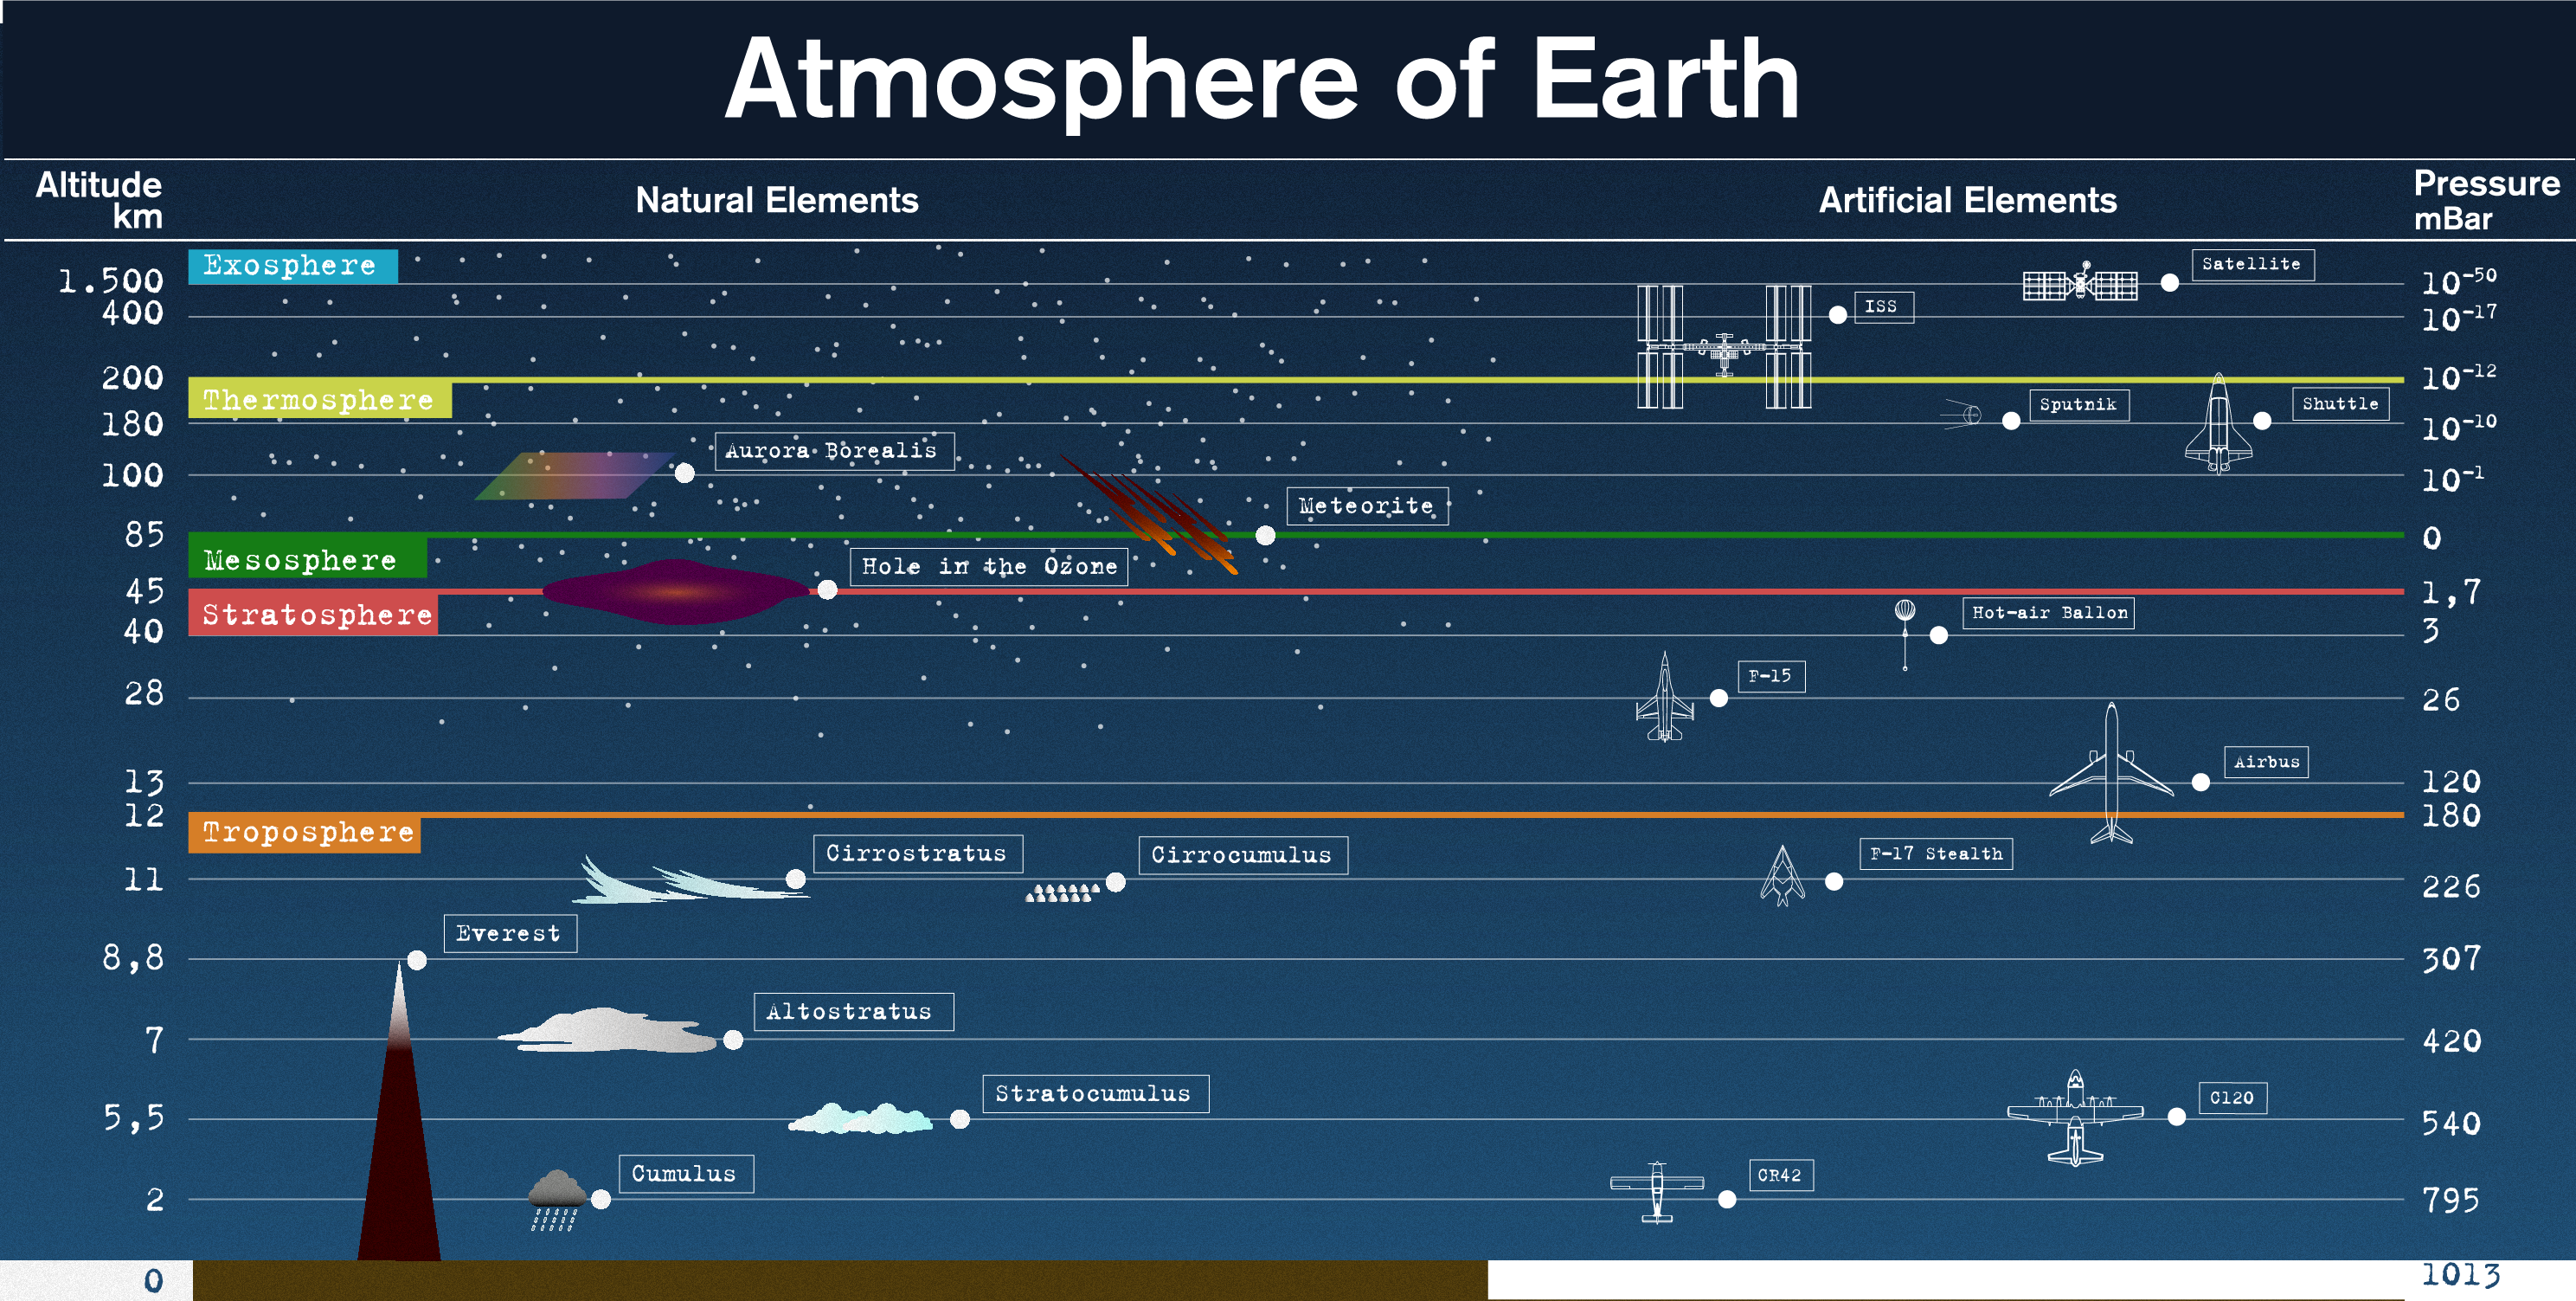
\includegraphics[width=15.0cm,height=10.0cm]{atmos2.png}
\end{figure}
La atmósfera es una capa de gases que rodea al planeta tierra y es retenida por la fuerza gravitacional ejercida por esta.
Esta protege la vida en la tierra creando presión para posibilitar la existencia del agua líquida en la superficie terrestre,absorbe la radiación ultravioleta emitida por el sol calentando la superficie através de la retención del calor y reduciendo las temperaturas extremas entre el día y la noche.


\subsection{Composición}

\begin{center}
    \begin{tabular}{| l | l | l | l |} \hline
   \multicolumn{2}{|l|}{\textbf{Gas}} &\multicolumn{2}{|c|}{\textbf{Volumen}}  \\ \hline
    Nombre & Fórmula & PPM & \% \\ \hline
    Nitrógeno & $N_2$ & 780,840 & 78.084 \\ \hline
    Óxigeno & $O_2$ & 209,460 & 20.946 \\ \hline
    Argón & Ar & 9,340 & .0934 \\ \hline
    Dióxido de Carbono & $CO_2$ & 400 & 0.04 \\ \hline
    Neón & Ne & 18.18 & 0.001818 \\ \hline
    Hélio & He & 5.24 & 0.000524 \\ \hline
    Metano & $CH_4$ & 1.79 & .000179 \\ \hline
  \hline
    \end{tabular}
\end{center}
\section{Estructura de La Atmósfera}
\begin{figure}[h!]
\centering
\includegraphics[width=5.0cm,height=7.0cm]{atmos.jpg}
\end{figure}

En general el aíre, la presión y la densidad decrecen con la altitud en la atmósfera.
La atmósfera de la tierra puede ser dividida en 5 capas principales las cuales se en listan  acontinuación de mayor a menor :
\begin{itemize}
\item \textbf{Exósfera}: 700 a 10,000 km (440 a 6,200 millas) \\
\\Esta capa se encuentra compuesta principalmente por hidrógeno y hélio extremadamente densos al igual que de moléculas de nitrógeno,oxígeno y dióxido de carbono extremadamente pesadas.\\
Los átomos y las moléculas están tan separadas que pueden viajar cientos de kilómetros sin colisionar unas con otras. \\
Por lo tanto, la exósfera tiende a comportarse como un gas \\ El movimiento libre de estas partículas sigue una trayectoria balística y pueden inmigrar a la magnetosfera o a los vientos solares.
\item \textbf{Termósfera}: 80 a 700 km (50 a 440 millas)
\\Esta capa es completamente nublada y libre de vapor de agua, de tal forma que ningún fenómeno hidro-meteorológico a excepción de las \textbf{Auroras Boreales} y las \textbf{Auroras Australianas} ocurren aquí.
Su altura varía considerablemente acorde a los cambios en la actividad solar porque la termopausa yace en la capa menor de la exosfera,también conocida como exobase.
La parte menor de la termósfera sobre la superficie terrestre contiene la Ionosfera.
La temperatura aquí incremente gradualmente con la altura, esta puede alcanzar hasta $1500^{\circ}$C ($2700^{\circ}$F).
\item \textbf{Mesósfera}: 50 a 80 km (31 a 50 millas)\\
la mesosfera es la tercera capa mas alta de la atmósfera de la tierra,Se extiende desde la estratopausa a una altitud de aproximadamente 50 km a la mesopausa a 80-85 km sobre el nivel del mar.\\
Las temperaturas descienden con el aumento de altitud hacia la mesopausa,que marca la parte superior de esta capa media de la atmósfera. \\
Es el lugar más frío de la Tierra y tiene una temperatura promedio de alrededor de $-85^\circ$C,
la mesosfera es tambien la capa donde la mayoria de los meteoros se queman al entrar en la atmosfera.
\item \textbf{Estratósfera}: 12 a 50 km (7 a 31 millas)\\
La estratosfera se extiende desde la parte superior de la Tropósfera hasta la estratopausa.
En esta las temperaturas aumentan de forma directamente con respecto a la altitud, esto es resultado de la absorción de los rayos UV en la capa de ozono.
\item \textbf{Troposfera}: 0 a 12 km (0 a 7 millas)\\
Esta se encuentra delimitada sobre la tropopausa, notable en las diferencias de temperatura.\\
Esta contiene aproximadamente 80\% de la masa de la atmósfera, siendo esta la más densa de las capas.
\end{itemize}
\section{Propiedades Físicas}
\subsection{Presión y densidad}
La presión atmosférica promedio a nivel del mar está definida por la \textbf{Atmósfera Estándar Internacional} como 101,325 pascales(atm).
Si toda la masa de la atmósfera tuviera una densidad uniforme desde el nivel del mar, terminaría abruptamente a una altitud de 8,50 km. \\
En realidad, disminuye exponencialmente con la altitud, disminuyendo a la mitad cada 5,6 km (18,000 pies) o por un factor de 1 cada cada 7,64 km.\\
Las diversas capas de la ionosfera de la Tierra, importantes para la propagación de la radio en ondas decamétricas, comienzan a menos de 100 km y se extienden más allá de 500 km.\\ Dependiendo de la actividad solar, los satélites pueden experimentar una resistencia atmosférica notable a altitudes de hasta 700-800 km.

\subsection{temperatura y velocidad del sonido}
La temperatura disminuye con la altitud comenzando al nivel del mar, pero las variaciones en esta tendencia comienzan por encima de los 11 km, donde la temperatura se estabiliza a través de una gran distancia vertical a través del resto de la troposfera.\\
La velocidad del sonido depende únicamente de la temperatura y no de la presión o densidad del gas,la velocidad del sonido en la atmósfera con la altitud adquiere la forma del perfil de temperatura complicado  y no refleja los cambios altitudinales en densidad o presión.
\subsection{Densidad y masa}
La densidad del aire a nivel del mar es de aproximadamente 1.2 kg/m$^{3}$, la densidad no se mide directamente, pero se calcula a partir de mediciones de temperatura, presión y humedad utilizando la ecuación de estado para el aire.

La masa promedio de la atmósfera es de aproximadamente 5 cuatrillones,La masa media total de la atmósfera es 5.1480$\times ^{algo}$ kg con un rango anual debido al vapor de agua de 1.2 o 1.5$\times ^{algo}$ kg, dependiendo de si se usan datos de presión superficial o vapor de agua algo más pequeña que la estimación anterior.

\section{propiedades ópticas}
La radiación solar,es la energía que recibe la Tierra del sol. La Tierra también emite radiación hacia el espacio, pero a longitudes de onda más largas que no podemos ver.
\subsection{Dispersión}
Cuando la luz pasa a través de la atmósfera de la tierra ,los fotones interactúan con ella a través de la dispersión. si la luz no interactúa con la atmósfera se le llama radiación directa, la radiación indirecta es la luz que se ha dispersado en la atmósfera
\subsection{Absorción}
\textbf{Diferentes moléculas absorben diferentes longitudes de onda de radiación.}\\
Los espectros de absorción combinados de los gases en la atmósfera dejan "ventanas" de baja opacidad, permitiendo la transmisión de solo ciertas bandas de luz.
\subsection{Emisión}
La emisión es lo opuesto a la absorción, es cuando un objeto emite radiación,los objetos más calientes tienden a emitir más radiación, con longitudes de onda más cortas. Los objetos más fríos emiten menos radiación, con longitudes de onda más largas.\\
Debido a su temperatura, la atmósfera emite radiación infrarroja. 
\subsection{Indice de refracción}
El índice de refracción del aire es cercano, pero apenas superior a 1. \\Las variaciones sistemáticas en el índice de refracción pueden conducir a la flexión de los rayos de luz en recorridos ópticos largos.
\section{Circulación}
La circulación atmosférica es el movimiento de aire a gran escala a través de la tropósfera, y de los medios, con circulación oceánica, por los cuales se distribuye el calor alrededor de la tierra.\\
\begin{figure}[h!]
\centering
\includegraphics[width=10.0cm,height=9.0cm]{circulacion.png}
\caption{circulación}
\end{figure}
\section{apendice}
\begin{itemize}
\item\textbf{¿Qué fue lo que más te llamó la atención de esta actividad?}\\
El saber acerca de la atmósfera terrestre, aprender a usar latex e investigar acerca de este.
\item\textbf{¿Qué fue lo que se te hizo menos interesante?}\\
lo largo del documente, pero de no ser extenso no se tendría la información precisa ya que se evitarían muchos temas.
\item\textbf{¿Qué cambios harías para mejorar esta actividad?}\\
Ninguno.
\item\textbf{¿Cuál es tu primera impresión de uso de LATEX?}\\
al inicio(semestre pasado) pensé que sería más difícil pero la verdad es solo cuestión de práctica y detener interés en aprender.
\item\textbf{¿El tiempo sugerido para esta actividad fue suficiente? }\\
Fue el suficiente.
\item\textbf{¿Encontraste algún documento o recurso en línea útil que quisieras compartir con los demás?}\\
La verdad me basé solo en el documento sugerido por el Maestro.
\end{itemize}
\section{Bibliografía}
wikipedia,29 de marzo del 2003,\textit{Atmosfera terrestre}
\end{document}
